% docs/latex/ef-impact.tex
\documentclass{standalone}
\usepackage{tikz}
\usetikzlibrary{arrows.meta,backgrounds}

\begin{document}
\pagecolor{white}
\color{black}
	\pagecolor{white}
	\color{black}
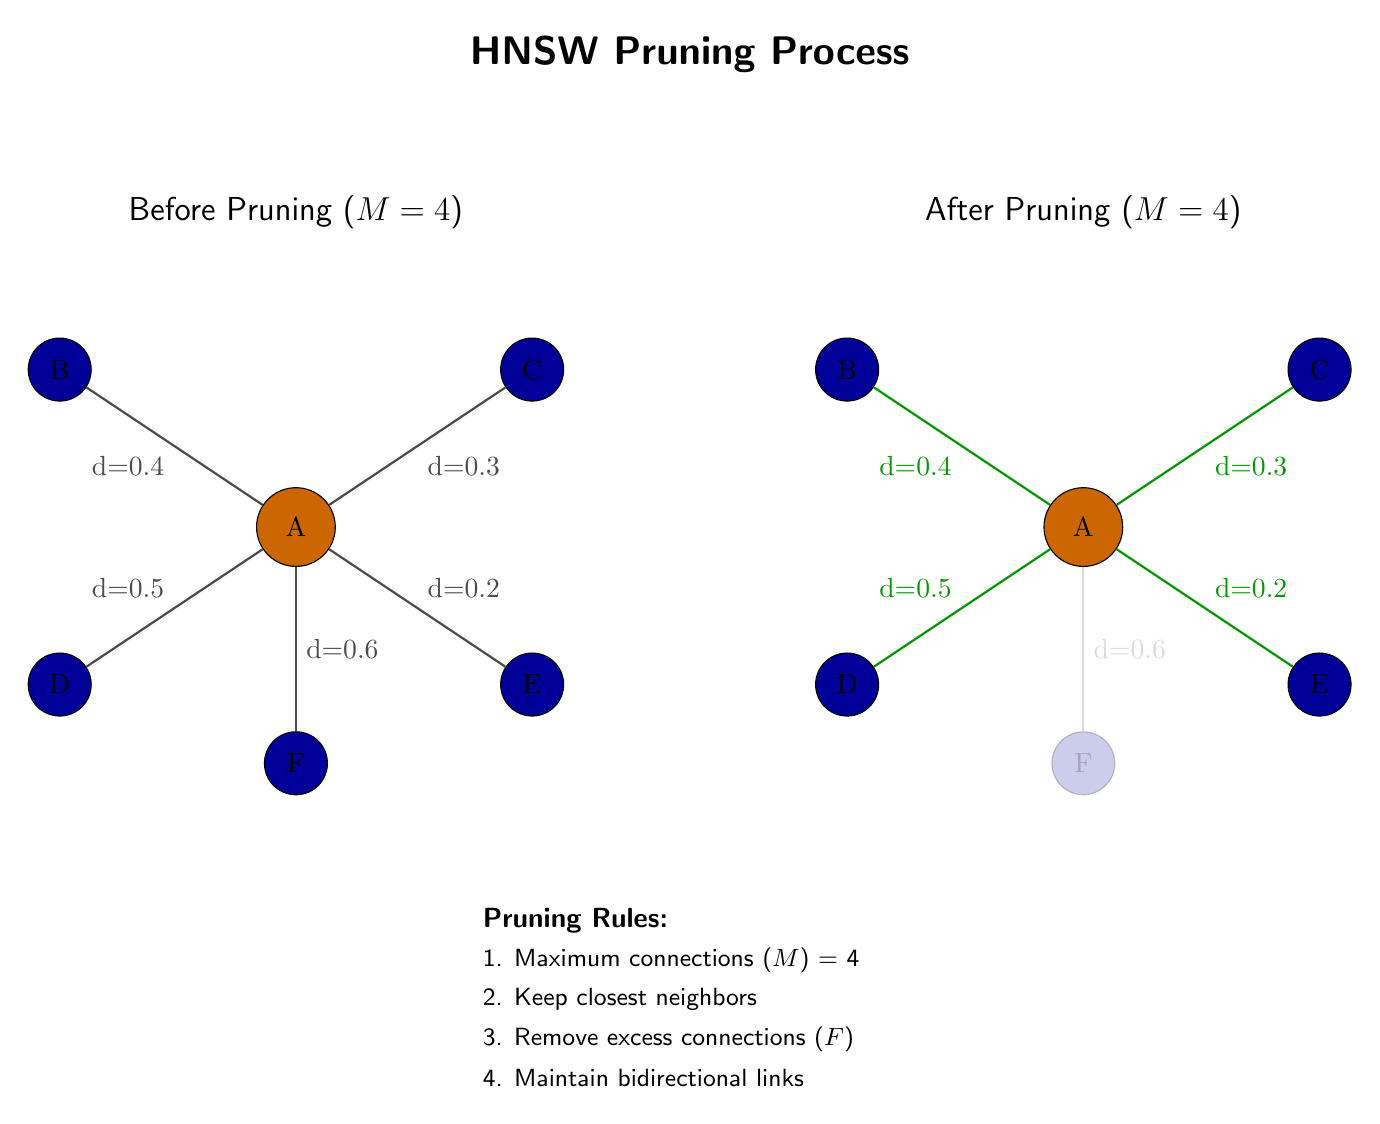
\begin{tikzpicture}[
    central node/.style={circle, draw, fill=orange!80!black, minimum size=1cm},
    normal node/.style={circle, draw, fill=blue!60!black, minimum size=0.8cm},
    faded node/.style={circle, draw, fill=blue!60!black, minimum size=0.8cm, opacity=0.2},
    connection/.style={-, thick, gray!60!black},
    kept connection/.style={-, thick, green!60!black},
    faded connection/.style={-, thick, gray!60!black, opacity=0.2},
    node label/.style={font=\sffamily},
    distance label/.style={font=\small\sffamily}
]

% Title
\node[font=\Large\sffamily\bfseries] at (0,6) {HNSW Pruning Process};

% Before Pruning
\begin{scope}[shift={(-5,0)}]
    \node[font=\sffamily\large] at (0,4) {Before Pruning ($M=4$)};
    
    % Central node
    \node[central node] (A1) at (0,0) {A};
    
    % Connected nodes
    \node[normal node] (B1) at (-3,2) {B};
    \node[normal node] (C1) at (3,2) {C};
    \node[normal node] (D1) at (-3,-2) {D};
    \node[normal node] (E1) at (3,-2) {E};
    \node[normal node] (F1) at (0,-3) {F};
    
    % Connections
    \draw[connection] (A1) -- (B1) node[midway, below left] {d=0.4};
    \draw[connection] (A1) -- (C1) node[midway, below right] {d=0.3};
    \draw[connection] (A1) -- (D1) node[midway, above left] {d=0.5};
    \draw[connection] (A1) -- (E1) node[midway, above right] {d=0.2};
    \draw[connection] (A1) -- (F1) node[midway, right] {d=0.6};
\end{scope}

% After Pruning
\begin{scope}[shift={(5,0)}]
    \node[font=\sffamily\large] at (0,4) {After Pruning ($M=4$)};
    
    % Central node
    \node[central node] (A2) at (0,0) {A};
    
    % Kept nodes
    \node[normal node] (B2) at (-3,2) {B};
    \node[normal node] (C2) at (3,2) {C};
    \node[normal node] (D2) at (-3,-2) {D};
    \node[normal node] (E2) at (3,-2) {E};
    \node[faded node] (F2) at (0,-3) {F};
    
    % Connections
    \draw[kept connection] (A2) -- (B2) node[midway, below left] {d=0.4};
    \draw[kept connection] (A2) -- (C2) node[midway, below right] {d=0.3};
    \draw[kept connection] (A2) -- (D2) node[midway, above left] {d=0.5};
    \draw[kept connection] (A2) -- (E2) node[midway, above right] {d=0.2};
    \draw[faded connection] (A2) -- (F2) node[midway, right, opacity=0.2] {d=0.6};
\end{scope}

% Pruning Rules
\node[font=\sffamily\bfseries, anchor=west] at (-2.75,-5) {Pruning Rules:};
\node[font=\small\sffamily, anchor=west] at (-2.75,-5.5) {1. Maximum connections ($M$) = 4};
\node[font=\small\sffamily, anchor=west] at (-2.75,-6.0) {2. Keep closest neighbors};
\node[font=\small\sffamily, anchor=west] at (-2.75,-6.5) {3. Remove excess connections ($F$)};
\node[font=\small\sffamily, anchor=west] at (-2.75,-7.0) {4. Maintain bidirectional links};

\end{tikzpicture}
\end{document}